\documentclass[adpaper,12pt]{book}
\usepackage[margin=24mm]{geometry}
\usepackage{graphicx}
\usepackage{float}
\usepackage{caption}
\usepackage{subcaption}
\geometry{bindingoffset=35mm}

\begin{document}

\title{Initial Project Proposal\\Skydive Formation Detection\\ (Dirt Dive Simulator)}
\author{Merlin Webster}
\date{}
\maketitle

\thispagestyle{empty}
\cleardoublepage
%\newpage



\section{Introduction}
	\subsection{Background}
Contrary to popular belief, skydiving is a competitive and technical sport, requiring careful control of body position in order to not only stay stable, but to move around the sky in freefall in a controlled manner.\\
A popular discipline in the sport is formation skydiving (FS). This involves multiple skydivers forming set formations in free-fall, in order to score as many points as possible. A point is awarded for each successful formation in a sequence \textbf{\emph{(see figure [\ref{fig:sample_fs}])}}.
%
\begin{figure}[H]
	\centering
	\begin{subfigure}{.33\textwidth}
		\centering
		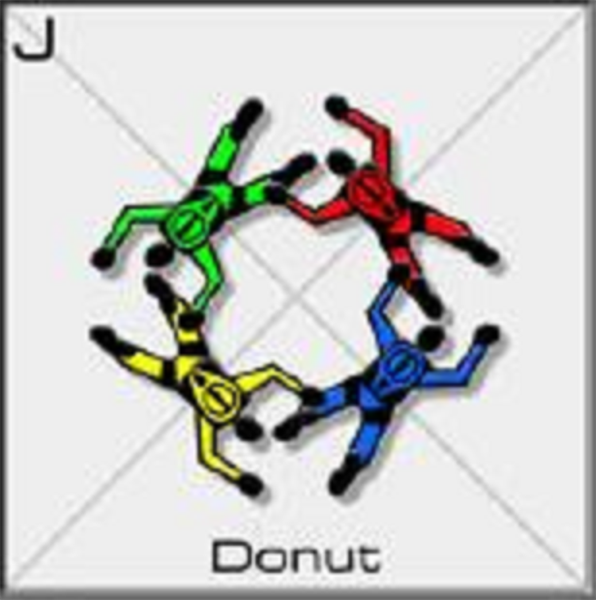
\includegraphics[width=0.9\linewidth]{FS_Donut.png}
	\end{subfigure}%
	\begin{subfigure}{.33\textwidth}
		\centering
		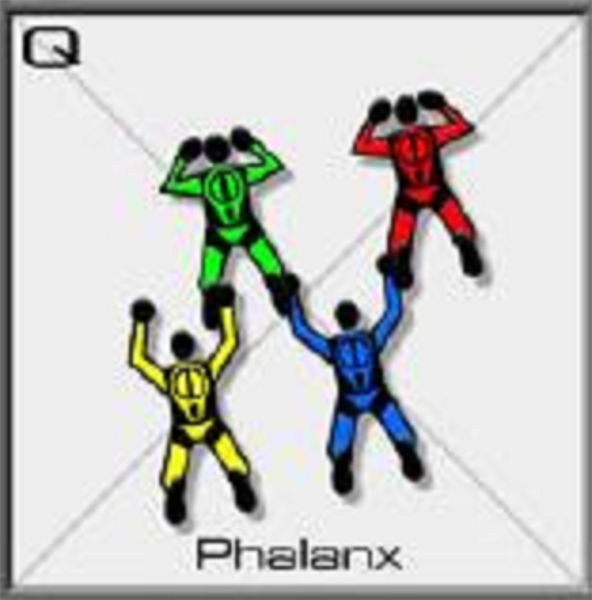
\includegraphics[width=0.9\linewidth]{FS_Phalanx.png}
	\end{subfigure}%
	\begin{subfigure}{.33\textwidth}
		\centering
		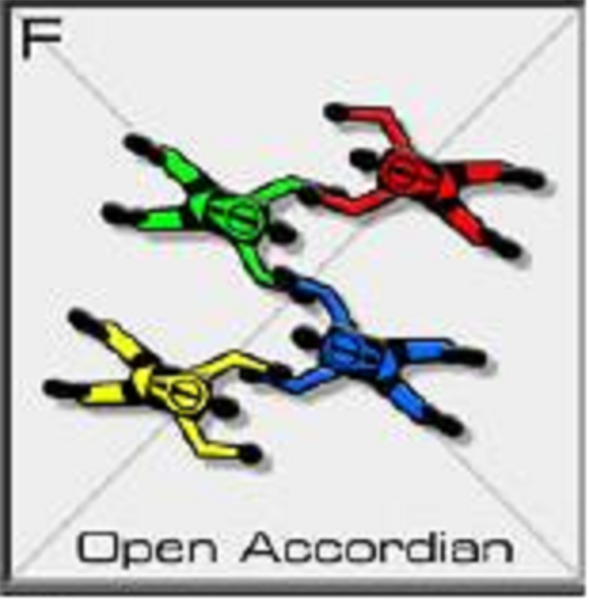
\includegraphics[width=0.9\linewidth]{FS_Accordian.png}
	\end{subfigure}\\
	\begin{subfigure}{.33\textwidth}
		\centering
		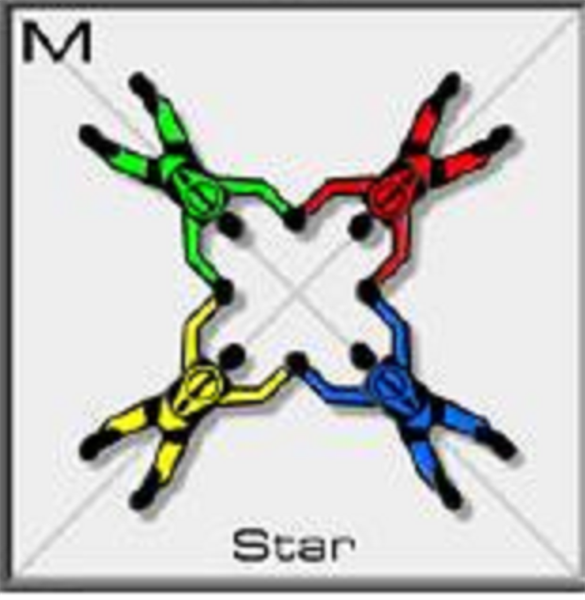
\includegraphics[width=0.9\linewidth]{FS_Star.png}
	\end{subfigure}%
	\begin{subfigure}{.33\textwidth}
		\centering
		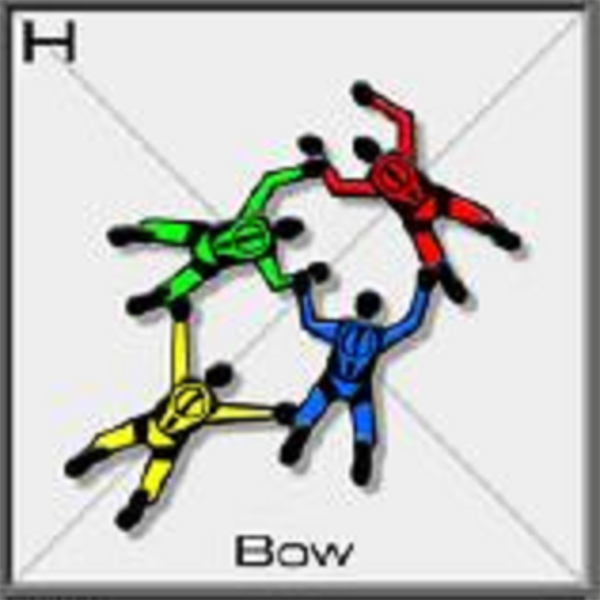
\includegraphics[width=0.9\linewidth]{FS_Bow.png}
	\end{subfigure}%
	\begin{subfigure}{.33\textwidth}
		\centering
		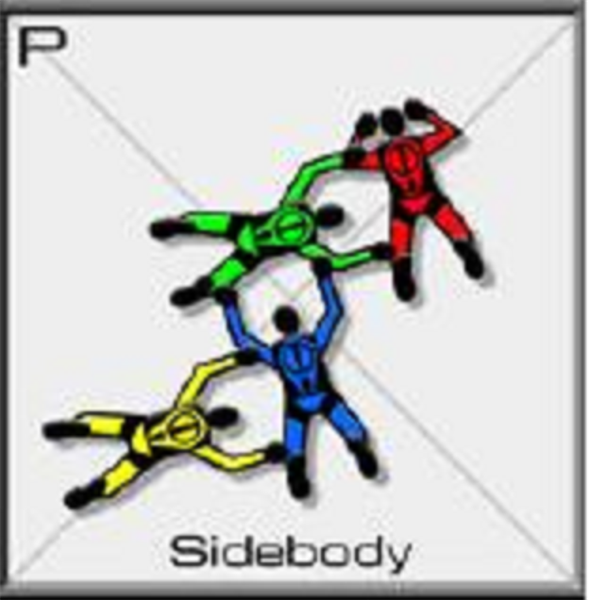
\includegraphics[width=0.9\linewidth]{FS_Sidebody.png}
	\end{subfigure}%
	\caption{Sample FS formations, with their names}
	\label{fig:sample_fs}
\end{figure}
%
In order for the team to create formations in the sky, it is important that they practice the skydive multiple times on the ground. This is known as "dirt diving" and is often done using partially triangular wheeled platforms that each skydiver lays on, known as "creepers"  \textbf{\emph{(see figures [\ref{fig:creepers}] and [\ref{fig:creepers_use}])}}.

\begin{figure}[H]
	\centering
	\begin{subfigure}{.5\textwidth}
		\centering
		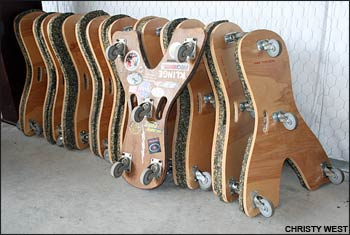
\includegraphics[width=0.9\linewidth]{creepers.jpg}
		\caption{FS practice platforms "creepers"}
		\label{fig:creepers}
		%http://www.skydivespaceland.com/blog/images/creepers2.jpg
	\end{subfigure}%
	\begin{subfigure}{.5\textwidth}
		\centering
		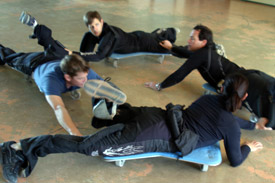
\includegraphics[width=0.9\linewidth]{creepers_use.jpg}
		\caption{"Creepers" in use while "dirt diving" a "Donut" formation}
		\label{fig:creepers_use}
		%http://www.skydiveaz.com/images/old-images/creepers.jpg?sfvrsn=2
	\end{subfigure}
	\caption{}
\end{figure}
%
	\subsection{Project Brief}
A system is proposed that would record the skydivers while dirt diving, analyse the video in real time and identify which formations they have formed.\\
The initial design could use a camera mounted directly above where the skydivers are dirt diving, but an angled wall mounted camera could possibly be used.
The video could then be streamed to a display, which would have have an overlay showing the positions of each of the skydivers, and what formation they are performing.
	
%
\section{Expandability Options}
	\subsection{In Air Formation Analysis}
	It is common practice for a cameraman to fly near a group of skydivers as they form formations, as a video is required for proof when judging FS competitions.
	If the video from the cameraman was when fed into a modified version of the software designed to analyse dirt diving, skydive could be autonomously judged, providing a run-down of the FS team's performance. This would provide a quick initial judging of the competition entry, without the need for a judge to watch the footage.

\end{document}